% lc*** Start of file template-TIF360-FYM360-blindtext.tex ******

% use on Overleaf!!!!
%
\documentclass[
 reprint,
 amsmath,amssymb,
 aps,
]{revtex4-2}

%\usepackage{stfloats}
\usepackage{caption}
\usepackage{dblfloatfix}
\usepackage{graphicx}% Include figure files
\usepackage{dcolumn}% Align table columns on decimal point
\usepackage{bm}% bold math
\usepackage[labelformat=simple]{caption}
\usepackage{hyperref}% add hypertext capabilities
%\usepackage[mathlines]{lineno}% Enable numbering of text and display math
%\linenumbers\relax % Commence numbering lines
\usepackage{xcolor}

\usepackage{lipsum}

\begin{document}

\title{[C] “Yeah, Right…”
	Sarcasm Classification on  Social Media}

\author{Arvid Kolstad}

\date{\today}% It is always \today, today,
%  but any date may be explicitly specified

\begin{abstract} %%% DO NOT CHANGE!
	%%% - B1 - %%%%%%%%%%%%%%%%%%%%%%%%%%%%%%%%%%% 
	%%% Customize this part: text between - B1 - and - E1 - must not appear in the final report 

	\noindent{Sarcasm} is a linguistically subtle phenomenon where the absence of prosodic cues makes automated detection particularly challenging. This project investigates three machine learning models, Logistic Regression, Bidirectional LSTM with multi-head attention, and BERTweet, trained to classify sarcastic comments drawn from a balanced Reddit dataset of one million entries. Logistic Regression serves as a baseline and performs only marginally above random chance, BiLSTM achieves a substantial improvement, and BERTweet attains the strongest performance, though it remains below state-of-the-art benchmarks. The results suggest that dataset noise from self-labeling and the absence of conversational context pose challenges that model capacity alone cannot fully overcome.
	%%% - E1 - %%%%%%%%%%%%%%%%%%%%%%%%%%%%%%%%%%%%%%

	\begin{description} %%% DO NOT CHANGE!
		\item[Project Topic] %%% DO NOT CHANGE!
		      {Sarcasm Detection in Social Media}
		\item[Teaching Assistant] %%% DO NOT CHANGE!
		      {Antonio Ciarlo} % CHANGE accordingly
	\end{description} %%% DO NOT CHANGE!
\end{abstract}

\maketitle




\section{\label{sec:intro}Introduction} %%% DO NOT CHANGE!

%%% - B2 - %%%%%%%%%%%%%%%%%%%%%%%%%%%%%%%%%%% 
%%% Customize this part: text between - B2 - and - E2 - must not appear in the final report 
\noindent{Human} communication is a rich and multifaceted phenomenon, shaped by tone, context, cultural background, and shared understanding between speakers. Among its many complexities, sarcasm stands out as a particularly challenging form of expression, one that relies heavily on non-verbal cues such as intonation, facial expression, and vocal emphasis to convey a meaning that is often the direct opposite of what is literally stated. While this poses little difficulty in face-to-face conversation, the written word strips away these contextual signals, leaving the reader to infer intent from text alone.

\noindent{This} challenge is amplified dramatically in the context of social media, where vast volumes of informal, unstructured text are produced daily across platforms dedicated to virtually every topic imaginable. On these platforms, sarcasm is not only common but often central to the culture of communication, used for humor, criticism, and commentary alike. The absence of prosodic cues in this medium means that sarcastic remarks are frequently misread, even by human readers familiar with the context.

\noindent{For} automated systems tasked with making sense of this content, whether for sentiment analysis, content moderation, or opinion mining, the accurate detection of sarcasm represents a significant open problem. A model that fails to recognize sarcasm will systematically misinterpret the sentiment and intent behind a large portion of online discourse, undermining the reliability of any downstream analysis.

\noindent{This} report investigates the capacity of machine learning models to address this problem by classifying sarcastic statements drawn from social media text. By evaluating and comparing different modeling approaches, this work aims to shed light on how well computational systems can grasp one of the more elusive dimensions of human language.

%%% - E2 - %%%%%%%%%%%%%%%%%%%%%%%%%%%%%%%%%%%%%%
\section{\label{sec:overview}Overview} %%% DO NOT CHANGE!
%%% - B3 - %%%%%%%%%%%%%%%%%%%%%%%%%%%%%%%%%%% 
%%% Customize this part: text between - B3 - and - E3 - must not appear in the final report
\noindent
In this section a brief summary of the models used in this report can be found. To every model, there is a short discussion about its advantages and weak point and an argument why the model was used.
\\ \\
\noindent
{\bf Method 1 - Logistic Regression.} \\{This model is rather simple and uses only a linear layer to classify the sentence from the vectorization. For this it uses the pre-trained model FastText \cite{grave2018learning} which is a more complex version of the famous Word2Vector. It can handle the problem of Out-Of-Vocabulary words by breaking up longer words into smaller parts that it does understand. This is great for social media text because of its higher frequency of typos and slang. Due to the models simplicity, it does not understand words connection to other words and therefore this is a good model to use as a benchmark.}
\\

\noindent
{\bf Method 2 BiLSTM with multi-head attention.} \\{This model uses a recurrent network that takes each word vector, both from the start of the sentence, and the end of the sentence, and feed these trough with the next word as input. After this the hidden states of the network gets fed into an attention network which learns how different words connects other. This is a good in between the Logistic Regression and the BERT-model and will hopefully display the importance of connections between words when it comes to classifying sarcasm.}
\\

\noindent
{\bf Method 3 BERT.}\\ {This model leans heavily on the pre-trained BERTweet model \cite{bertweet}, and leverages its understanding of language to try to predict sarcasm. The BERTweet is a transformer encoder that first has been trained on a big dataset of english, and then have been fine tuned on 850 million tweets. This makes it good at understanding internet language and slang, which makes it perfect for this classification problem. It's without question the biggest model in this project and has over 100 million parameters, and has the best chances of scoring the highest.}

\onecolumngrid
\begin{center}
	\captionof{table}{{\bf Overview of ML models used in this project.} Table where the different models used in the project is presented, their features explained and arguments for their fit to the project.
	}
	\label{tab:methodsoverview}
	\begin{tabular}{| l | l | l | l |}
		\hline
		\parbox[t]{1.8cm}{
			{\bf Method }
		}              &
		\parbox[t]{4cm}{
			{\bf Use case scenario }
		}              &
		\parbox[t]{5.5cm}{
			{\bf Features }
		}              &
		\parbox[t]{5.5cm}{
			{\bf Suitable for the project? }
		}                \\
		\hline
		\hspace{0.1cm}
		\parbox{1.8cm}{\begin{flushleft}
				               Logistic regression
			               \end{flushleft}}
		\hspace{0.1cm}
		               &
		\hspace{0.1cm}
		\parbox{2.8cm}{\begin{flushleft}
				               Classification Model
			               \end{flushleft}}
		\hspace{0.1cm}
		               &
		\hspace{0.1cm}
		\parbox{5.5cm}{\begin{flushleft}
				               Fast and simple model that is easy to interpret and train. Looks at the importance of each word in the sentence to classify it. Probably too simple for classifying harder sentences.
			               \end{flushleft}}
		\hspace{0.1cm}
		               &
		\hspace{0.1cm}
		\parbox{5.5cm}{\begin{flushleft}
				               Well studied method that is used for getting a base line performance on the data set.
			               \end{flushleft}}
		\hspace{0.1cm}
		\\
		\hline
		\hspace{0.1cm}
		\parbox{1.8cm}{\begin{flushleft}
				               BiLSTM with multi-head attention
			               \end{flushleft}}
		\hspace{0.1cm}
		               &
		\hspace{0.1cm}
		\parbox{2.8cm}{\begin{flushleft}
				               Classification Model
			               \end{flushleft}}
		\hspace{0.1cm} &
		\hspace{0.1cm}
		\parbox{5.5cm}{\begin{flushleft}
				               Can capture word order and connect words over larger distances in sentences which is important for sarcasm. The attention mechanism can learn what words refers to each other and therefore understand the sentence better.
			               \end{flushleft}}
		\hspace{0.1cm}
		               &
		\hspace{0.1cm}
		\parbox{5.5cm}{\begin{flushleft}
				               Medium size model that had great performance for its time.
			               \end{flushleft}}
		\hspace{0.1cm}
		\\
		\hline
		\hspace{0.1cm}
		\parbox{1.8cm}{\begin{flushleft}
				               BERTweet
			               \end{flushleft}}
		\hspace{0.1cm}
		               &
		\hspace{0.1cm}
		\parbox{2.8cm}{\begin{flushleft}
				               Classification Model
			               \end{flushleft}}
		\hspace{0.1cm} &
		\hspace{0.1cm}
		\parbox{5.5cm}{\begin{flushleft}
				               An already pre-trained language model that can be used to classify sarcasm by setting a linear layer after it and fine-tuning the whole model on the specific data set. The model is quite large and therefore it can be computationally intensive to train.
			               \end{flushleft}}
		\hspace{0.1cm}
		               &
		\hspace{0.1cm}
		\parbox{5.5cm}{\begin{flushleft}
				               A large model that has a good understanding of our language, which makes it perfect for using in this classification problem.

			               \end{flushleft}}
		\hspace{0.1cm}
		\\
		\hline
	\end{tabular}
\end{center}
\twocolumngrid


%%% - E3 - %%%%%%%%%%%%%%%%%%%%%%%%%%%%%%%%%%%%%%



\section{\label{sec:method}Method} %%% DO NOT CHANGE!
%%% - B4 - %%%%%%%%%%%%%%%%%%%%%%%%%%%%%%%%%%% 
%%% Customize this part: text between - B4 - and - E4 - must not appear in the final report
In this section we will first introduce the dataset and then we will go through the different models architecture and then explain the training pipeline. All the models are built in python by using the library PyTorch.
\subsection{Dataset}
The dataset that has been used in this project is the following \cite{SARC}. It's a dataset that was retrieved from the website Kaggle.com, and has been created by scraping the the social platform Reddit.com for comments. On the website you can put different labels on your comments to signal what the comment is about. One of these labels stands for that the comment has some sarcastic remarks in it, and this is what is used for classifying the dataset.The total number of comments is exactly 1 million and the dataset is perfectly balanced so 500K is labeled as normal and the other half is labeled as sarcastic. The dataset also contained the text that the comment answered to, what the authors name was, the name of the specific chat forum that the comment was written in and much more but the only data that was used in this project was the original comment and its sarcasm label.
\subsection{FastText}
For both this model and the BiLSTM, the word embedding tool FastText is used \cite{grave2018learning}. It is a pre trained model that takes a word and transforms it into a 300 dimensional vector, and therefore makes it easier interpretable to a computer. This model was picked for the project for its ability to handle Out-Of-Vocabulary words. If it stumbles upon a word that it doesn't recognize it tries to break down the word in smaller words that could make the word make sense. This is great for handling slang and spelling error that might not be included in the FastText set of known words. This model only handles word so special characters are removed before converting the word to a sentence. For sarcasm in text, these provide valuable markers so to not loose this information, 4 sarcasm pointer where extracted from each sentence. The pointers where words with where all letters where capitalized, and the sequences "!!!, "?!" or "!?", and "...". Other papers like \cite{9420094} and \cite{KumarEtAl2021} use more sarcasm pointers with higher complexity than what's used in this project, but with regards to time scope of the project it was decided that these four pointers where enough.
\subsection{Logistic Regression}
\noindent
This model serves as the simplest baseline and is expected to face challenges in capturing the nuances of sarcasm. Because the comments vary in length, and the logistic regression model requires a fixed-size input, a mean sentence vector was computed by averaging the FastText embeddings of all words within a given comment. A consequence of this pooling approach is that the model can only capture the global semantic theme of the comment, while all sequential relationships and syntactic dependencies between words are lost. This sentence vector is subsequently concatenated with the sarcasm pointers and fed through a linear layer to produce a single scalar value. Finally, classification is performed using a sigmoid activation function applied against a specified threshold. A comprehensive flowchart of this baseline architecture is illustrated in Figure \ref{fig:selectedmethod}.

\subsection{BiLSTM with Multi-Head Attention}
\noindent
This architecture is highly inspired by the work of \cite{KumarEtAl2021}, with the primary modification being the inclusion of fewer sarcasm pointers. In contrast to the Logistic Regression baseline, words are first mapped to vectors using FastText to construct a sequence matrix, preserving the individual word vectors rather than averaging them.
\\ \\
This sequence is then fed into a Bidirectional Long Short-Term Memory (BiLSTM) network. The bidirectional nature ensures that the network processes the text both forward (from the first to the last word) and backward (from the last to the first word), generating two distinct hidden states at each time step. Consequently, the hidden state representation of a specific word is influenced by both its preceding and succeeding context.
\\ \\

The complete set of hidden state vectors from both directions is subsequently passed to an attention layer to compute self-attention weights. This is achieved by passing the hidden states through two linear layers interspersed with a hyperbolic tangent ($\tanh$) activation function, followed by a softmax function to normalize the weights. Lastly, these weights are multiplied by the original hidden vectors, and the resulting matrix is flattened and concatenated with the sarcasm pointers. A final linear layer is then utilized for the final classification. The corresponding flowchart for this model is detailed in Figure \ref{fig:selectedmethod}.


\onecolumngrid
\begin{center}

	\captionsetup{type=figure}
	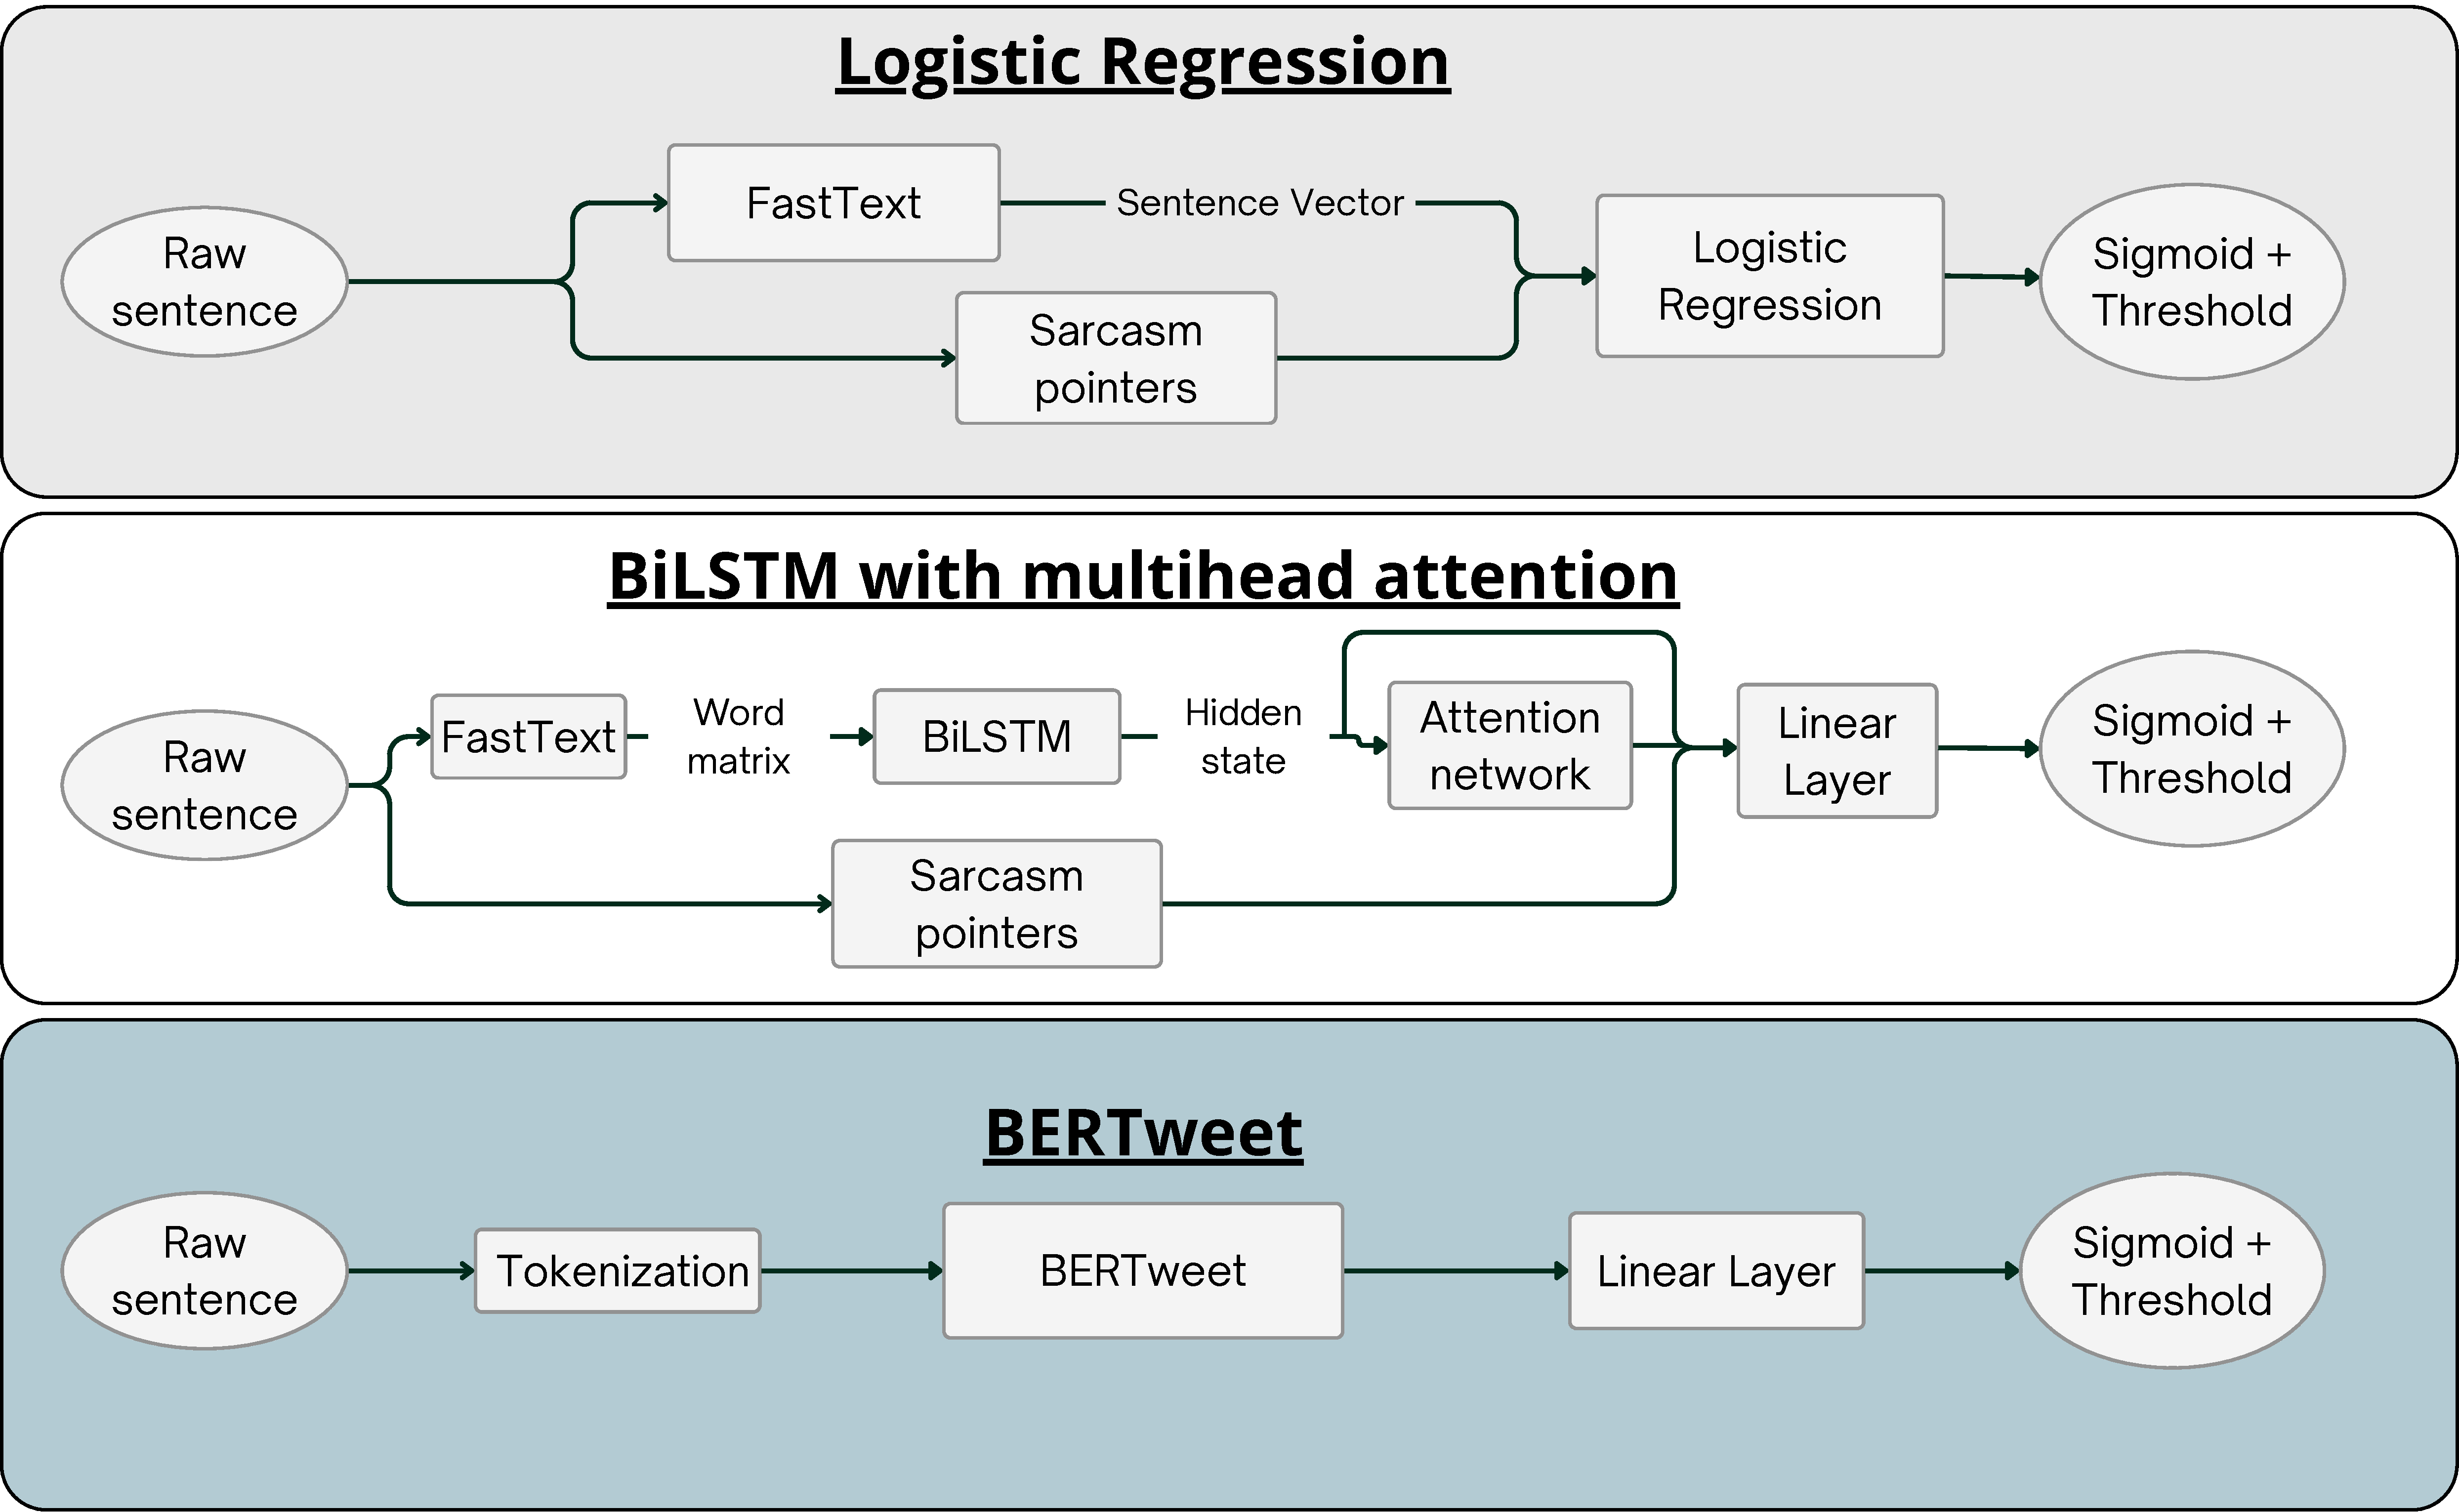
\includegraphics[width=0.89\textwidth]{figures/Flowchart Whiteboard in Bright Green Lime Green Pink Corporate Neon Style.pdf}

	\captionof{figure}{{\bf Flowchart of the models used in the project:}
		Architectural comparison of three sarcasm detection models. Top: a Logistic Regression baseline combining FastText sentence vectors and sarcasm pointers. Middle: a BiLSTM with multihead attention, using FastText word embeddings and sarcasm pointers as input. Bottom: a BERTweet transformer model with tokenization and a linear layer. }
	\label{fig:selectedmethod}


\end{center}
\clearpage

\twocolumngrid
\subsection{BERTweet}
\noindent
To leverage a large-scale pre-trained language model, a BERTweet architecture \cite{bertweet} was implemented and fine-tuned for the sarcasm classification task. Unlike the previous models, additional explicit sarcasm pointers were omitted for this configuration; the specialized BERTweet tokenizer natively retains and processes emojis, hashtags, and special characters, allowing the model to encode these stylistic cues implicitly.
\\ \\
Instead of generating static embeddings or processing sequences through recurrent layers, the input tokens are passed through the transformer blocks to capture deep, bidirectional contextual representations. For the final classification task, the embedding of the special classification token (\texttt{[CLS]}), which aggregates the semantic representation of the entire sequence, is extracted from the final hidden layer. This token embedding is then fed directly into a final linear layer to project the representation to a single logit, which is subsequently classified using a sigmoid function and a threshold. The architectural overview of this fine-tuned model is presented in Figure \ref{fig:selectedmethod}.
\noindent

\subsection{Model and Training configuration}
\noindent
The dataset was divided into three different sets: Training ($50\%$), Validation ($25\%$) and Test ($25\%$) where the class balance where kept. The training set was used to train the models parameters, the validation set was used for stopping training and also to set the final threshold by iterating over each threshold and picking the best one, and the test set was used to get the results. The total parameter in the Logistic Regression is 304 parameters, while the BiLSTM contains 474 629 parameters and last but not least the BERTweet with 134 900 737 parameters.

%\fbox{\parbox[t][][t]{\columnwidth}{
%\textbf{Points:} \fbox{\bf \textcolor{magenta}{8}} out of \textbf{44}

%Provide here the details of the method you have chosen for the project.
%You should explain and provide enough detail such that your results can be reproduced following your method.
%Compose a figure that contains / describes your method (mandatory). Refer to the figure (Fig.~\ref{fig:selectedmethod}) when describing the method in the text.
%You can add a second figure if you believe it is necessary.
%}
%%- E4 - %%%%%%%%%%%%%%%%%%%%%%%%%%%%%%%%%%%%%%





\section{\label{sec:results}Results and Discussion} %%% DO NOT CHANGE!
%%% - B5 - %%%%%%%%%%%%%%%%%%%%%%%%%%%%%%%%%%%
%%% Customize this part: text between - B5 - and - E5 - must not appear in the final report
\noindent
In this section the results are presented and discussed. Table \ref{tab:results} shows the accuracy and F1-score for each model. Logistic Regression performs only marginally above random chance, which is expected given the model's limited capacity for capturing contextual information. BiLSTM with multi-head attention achieves a substantial improvement, performing comparably to the model proposed by \cite{KumarEtAl2021}. BERTweet achieves the highest performance of the three models; however, it falls notably short of state-of-the-art results reported in \cite{SharmaEtAl2026}. This gap may be attributed to several factors, including computational constraints and dataset quality. The dataset was constructed by scraping Reddit posts where users self-labeled their comments as sarcastic, which introduces noise — there is no guarantee that sarcastic comments without such labels were excluded from the non-sarcastic class.

\begin{table}[]
	\begin{tabular}{|c|c|c|c|}
		\hline
		\textbf{Method}                                                & \textbf{Accuracy} & \textbf{F1-Score} & \textbf{Threshold} \\ \hline
		\begin{tabular}[c]{@{}c@{}}Logistic \\ Regression\end{tabular} & 0.580             & 0.680             & 0.380              \\ \hline
		BiLSTM                                                         & 0.702             & 0.732             & 0.320              \\ \hline
		BERTweet                                                       & 0.779             & 0.792             & 0.330              \\ \hline
	\end{tabular}
	\caption{Results for the three models. Logistic Regression is just better than guessing random. BiLSTM makes a big jump up on both accuracy and F1-Score, but BERTweet is still far better. We can also see that for all the models the thresholds are all low.}
	\label{tab:results}
\end{table}
\begin{centering}
	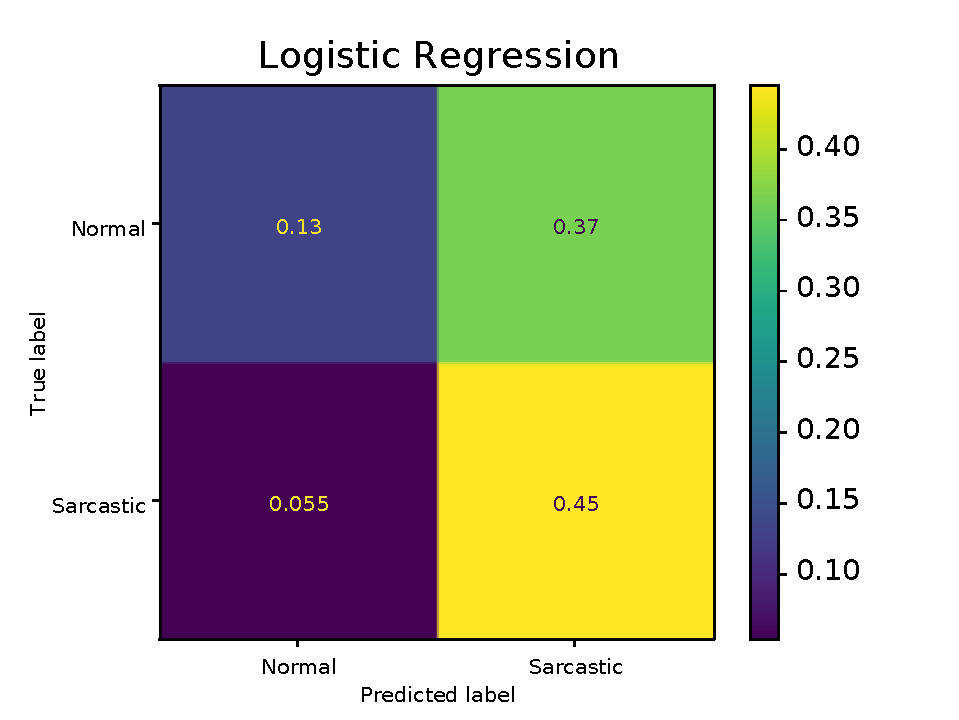
\includegraphics[width=0.94\columnwidth]{figures/logreg_confusion_matrix.pdf}
	\captionof{figure}{{\bf Confusion Matrix for Logistic Regression} In the figure we can see how the model almost always guesses sarcastic, which signals that this model architecture can not understand sarcasm.}
	\label{fig:logreg_confusion_matrix}
\end{centering}
\begin{centering}
	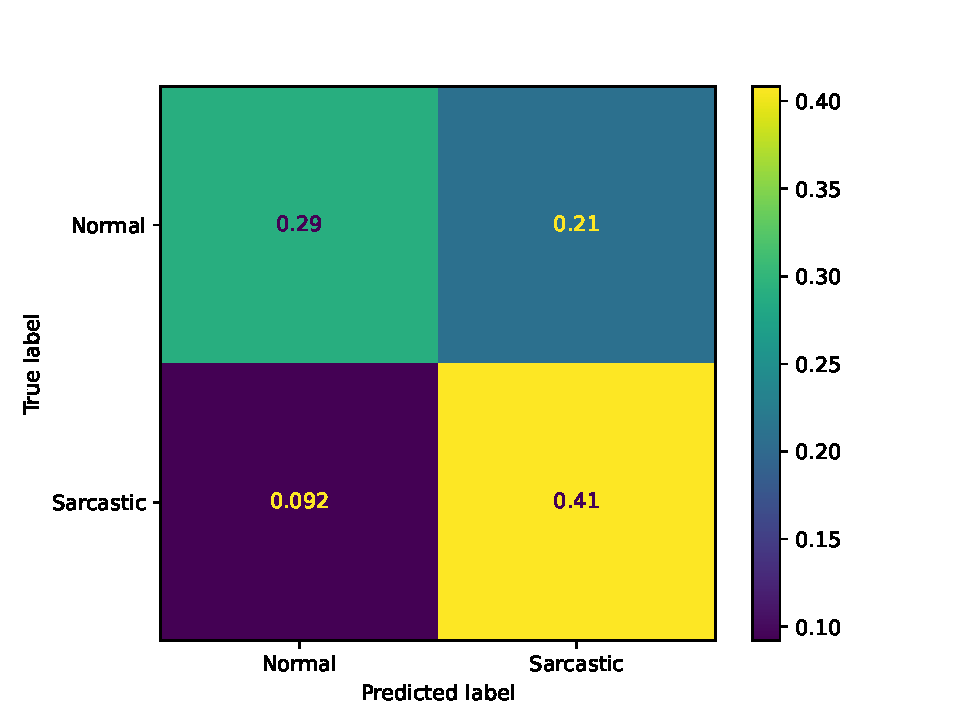
\includegraphics[width=0.94\columnwidth]{figures/LSTM_confusion_matrix.pdf}
	\captionof{figure}{{\bf Confusion Matrix for BiLSTM} The BiLSTM performs better and the classifications are more balanced, but still overestimates the sarcastic classifications.}
	\label{fig:bilstm_confusion_matrix}
\end{centering}
\begin{centering}
	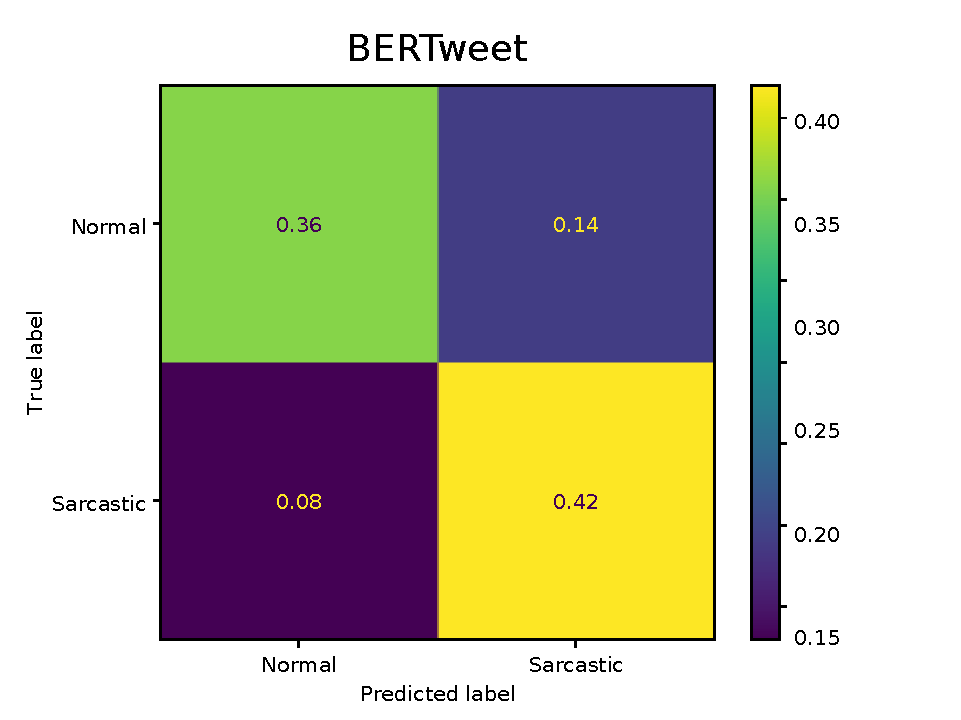
\includegraphics[width=0.94\columnwidth]{figures/BERTweet_confusion_matrix.pdf}
	\captionof{figure}{{\bf Confusion Matrix fot BERTweet} The best performing model and which also has the best balance between sarcastic and normal classifications.}
	\label{fig:BERTweet_confusion_matrix}
\end{centering}
\noindent
The confusion matrices reveal the classification strategy adopted by each model. As shown in figure \ref{fig:logreg_confusion_matrix}, Logistic Regression defaults to predicting sarcasm for the majority of inputs, reserving the non-sarcastic class only for high-confidence cases. Figure \ref{fig:bilstm_confusion_matrix} demonstrates that BiLSTM produces considerably more balanced predictions, suggesting that the self-attention mechanism meaningfully improves the model's ability to detect sarcastic language. Figure \ref{fig:BERTweet_confusion_matrix} shows the most balanced classification of the three, with false positive and false negative rates approaching parity. Notably, all models converge on a similar optimal threshold well below 0.5, despite being trained with a threshold of 0.5 that was subsequently adjusted using validation data. This consistent pattern suggests that sarcastic signals in the data are weak, and that models tend to assign low-confidence probabilities even to genuinely sarcastic samples. One possible explanation is that the self-labeling nature of the dataset introduces noise into the sarcastic class, causing models to assign cautiously low probabilities across the board. A reduced threshold is then necessary to recover meaningful recall, consistent with the general bias toward sarcastic predictions seen across all confusion matrices.



\section{\label{sec:conclusion}Conclusions and Outlook} %%% DO NOT CHANGE!
\noindent
Logistic Regression demonstrates limited capacity for reliable sarcasm detection, while BiLSTM and BERTweet both achieve considerably stronger performance given the constraints of the dataset. A potential avenue for improvement would be to incorporate contextual information, such as the parent post to which a comment responds, as sarcasm is often dependent on the broader conversational context. This is particularly relevant for short social media comments, where the absence of such context makes classification challenging even for human annotators.
%%% - B6 - %%%%%%%%%%%%%%%%%%%%%%%%%%%%%%%%%%% 
%%% Customize this part: text between - B6 - and - E6 - must not appear in the final report 

%%% - E6 - %%%%%%%%%%%%%%%%%%%%%%%%%%%%%%%%%%%%%%





\section{\label{sec:Contribution}Contributions} %%% DO NOT CHANGE!


%%% - B7 - %%%%%%%%%%%%%%%%%%%%%%%%%%%%%%%%%%% 
%%% Customize this part: text between - B7 - and - E7 - must not appear in the final report 
%\noindent
%\fbox{\parbox[t][][t]{\columnwidth}{
%\textbf{Points:} \fbox{\bf \textcolor{magenta}{1}} out of \textbf{44}

%Mandatory in all cases (also in the case of 1-person team).

%Add some text. See a possible text below.
%}}
\noindent
Kolstad, A. conceived and implemented the code for the project. Kolstad, A. created the poster for the presentation of the project. Kolstad, A. wrote the report for the project.
%Example: A.B. and C.D. conceived and implemented ... (adapt). E.F., G.H., contributed to .... etc etc. All authors ... (adapt).
%%% - E7 - %%%%%%%%%%%%%%%%%%%%%%%%%%%%%%%%%%%%%%



\section{\label{sec:COI}Conflict of Interest} %%% DO NOT CHANGE!

%%% - B8 - %%%%%%%%%%%%%%%%%%%%%%%%%%%%%%%%%%% 
%%% Customize this part: text between - B8 - and - E8 - must not appear in the final report 
\noindent
The author declare that they have no known competing financial interests or personal relationships that could have appeared to influence the work reported in this paper.
\noindent
%\fbox{\parbox[b][][t]{\columnwidth}{
%\textbf{Points:} \fbox{\bf \textcolor{magenta}{1}} out of \textbf{44}

%Add some text. See a possible text below.
%}}

%{{\bf Note:} A conflict of interest can also be known as {\emph competing interest}. A conflict of interest can occur when you, or your employer, or sponsor have a financial, commercial, legal, or professional relationship with other organizations, or with the people working with them, that could influence your research.
%For example check here:} \href{https://authorservices.taylorandfrancis.com/editorial-policies/competing-interest/}{https://authorservices.taylorandfrancis.com/editorial-policies/competing-interest/}
%%% - E8 - %%%%%%%%%%%%%%%%%%%%%%%%%%%%%%%%%%%%%%




\section{\label{sec:datacode}Data and Code Availability} %%% DO NOT CHANGE!
The code can be found at:\url{ https://github.com/ArvidKolstad/Advanced-Neutal-Network} and the dataset can be found at \url{https://www.kaggle.com/datasets/danofer/sarcasm/data}
%%% - B9 - %%%%%%%%%%%%%%%%%%%%%%%%%%%%%%%%%%% 
%%% Customize this part: text between - B9 - and - E9 - must not appear in the final report 
\noindent
%\fbox{\parbox[b][][t]{\columnwidth}{
%\textbf{Points:} \fbox{\bf \textcolor{magenta}{1}} out of \textbf{44}

%Add some text. See a possible text below.
%}}

%Data is available for download at ....  / can be accessed from ....

%All source code and examples are made publicly available at ... . The version used in this study is archived in ... with DOI ...
%%% - E9 - %%%%%%%%%%%%%%%%%%%%%%%%%%%%%%%%%%%%%%



%%% - B10 - %%%%%%%%%%%%%%%%%%%%%%%%%%%%%%%%%%% 
%%% Customize this part: text between - B10 - and - E10 - must not appear in the final report 
\noindent




\bibliography{biblio-TIF360-FYM360}

\end{document}
